%
% This template has been created by:
% Pascal Bercher, pascal.bercher@anu.edu.au
%
% This is version 1.00 (3. Dec. 2021)
% Make sure to use the newest version available on git:
%
% I was too lazy to put it under a specific license, but you are still free to use and alter it.
% But since I put a *lot* of effort (and experience)

\documentclass[a4paper,twoside,cleardoublepage=plain,bibliography=totoc]{scrbook}

\usepackage[a4paper]{geometry}                    % used for defining the title page

\usepackage{xurl}                                 % allows long URLs to break at any position
\usepackage[backref=page]{hyperref}               % defines style of references / links
\hypersetup{
linktocpage,                                      % in the table of contents, the numbers serve as links, not the entries
colorlinks  = true,                               % the items are colored instead of colored boxes around them
urlcolor    = cyan,
linkcolor   = red,
citecolor   = blue
}
% the following makes back references more appealing.
% Taken from: https://tex.stackexchange.com/questions/183702/formatting-back-references-in-bibliography-bibtex
\renewcommand*{\backref}[1]{}
\renewcommand*{\backrefalt}[4]{[%
\ifcase #1 Not cited.%
  \or Cited on page~#2.%
  \else Cited on pages #2.%
\fi]}




\usepackage{datetime}                             % to be able to print month & year on title page
\usepackage{amssymb,amsthm,amsmath}               % standard math packages; often used
\usepackage{graphicx}                             % allows including graphics
\usepackage{natbib}                               % a specific citation style
\usepackage{floatrow}                             % allows to place a caption next to a figure
  \floatsetup[table]{capposition=top}             %  forces table captions to appear on top.
\usepackage{booktabs}                             % for tables that actually look nice!
\usepackage{paralist}                             % provides compactitem, a more compact itemize
\usepackage{titlesec}                             % used to add those horizontal lines around chapter package; see defs below.
\usepackage[standardsections]{scrhack}            %  fixes an error causes by loading titlesec for class scrbook
\usepackage{parskip}                              % when this is included, no indentations are used for new paragraphs,
                                                  % and instead paragraphs are separated by a small distance between them


% [requires titlesec]
% Surrounds all chapter titles by lines (see screenshot),
% which includes the titles in the TOC and list of figures and tables
\titleformat{\chapter}[display]
{\bfseries\huge}
{\filleft\Large\chaptertitlename~\thechapter}
{3ex}
{\titlerule\vspace{1.5ex}\filright}
[\vspace{1ex}\titlerule]

% fixes a compilation errror that otherwise occurs in combination with scrbook
% see https://tex.stackexchange.com/questions/625083/adding-horizontal-line-before-and-after-chapter-heading-in-scrbook
% \titleformat{\section}
%  {\normalfont\Large\bfseries}{\thesection}{1em}{}
% \titleformat{\subsection}
%  {\normalfont\large\bfseries}{\thesubsection}{1em}{}
% \titleformat{\subsubsection}
%  {\normalfont\normalsize\bfseries}{\thesubsubsection}{1em}{}
 

 

% !! Set your individual data for the title page
%    in the configuration file !!

% Set your name:
%  (Well, your name.)
\newcommand{\AuthorName} {Ying Xian Wu}


% Set the title of your work:
%  (Choose an informative and interesting title.)
\newcommand{\ProjectTitle} {Transforming Partially Ordered Planning Problems into Totally Ordered Problems}


% Set which titlepage layout you prefer. Both provide the exact same
% information, they only differ in design to give you a bit of individuality
%  (change second line accordingly)
\newif\ifStandardTitle % do not delete this part!
\StandardTitletrue     % or \StandardTitlefalse or comment out


% Set the name of your school:
%  (School of Computing, School of Engineering,
%   or School of Cybernetics)
\newcommand{\School} {School of Computing}


% Set the name of your college:
%  (However your College is called.)
\newcommand{\College} {College of Engineering and Computer Science (CECS)}


% Set your project points:
%  (6 or 12 or 24)
\newcommand{\ProjectPoints} {24}


% Set whether it's an Honours thesis:
%  (change second line accordingly)
\newif\ifHonoursThesis % do not delete this part!
\HonoursThesistrue     % or \HonoursThesisfalse or comment out


% Set your semester:
%  (S1 or S2 or S1/S2 or S2/S1 or Summer)
\newcommand{\Semester} {S1/S2}


% Set your year:
%  (YYYY or YYYY--YYYY in case of S2/S1)
\newcommand{\Year} {2022}


% Set your degree:
%  (Whatever your degree is called.)
%  (Only required if Honours = true)
\newcommand{\Degree} {Bachelor of Advanced Computing}


% Set your course code and name:
%  (Whatever your course code and name is.)
%  (Only required if Honours = false)
\newcommand{\CourseCode} {COMP4540}
\newcommand{\CourseName} {Software Engineering Research Project}


% Set name of first supervisor:
%   (Whatever her or his name is.)
\newcommand{\FirstSupervisor} {Dr.\ Pascal Bercher}


% Set whether there's a second supervisor:
%  (change second line accordingly)
\newif\ifTwoSupervisors % do not delete this part!
\TwoSupervisorstrue     % or \TwoSupervisorsfalse or comment out


% Set name of second supervisor:
%  (Whatever her or his name is.)
%  (Only required if TwoSupervisors = true)
\newcommand{\SecondSupervisor} {Mr.\ Songtuan Lin}
                             % to specify data used in the title page

% define your own macros here

\newcommand{\Eff} {\ensuremath{\mathit{eff}}}  % example command without arguments
\newcommand{\Pre} {\ensuremath{\mathit{pre}}}  % (again)
\newcommand{\Add} {\ensuremath{\mathit{add}}}
\newcommand{\Del} {\ensuremath{\mathit{del}}}
\newcommand{\PreS} {\ensuremath{\mathit{pre^{*}}}}
\newcommand{\AddS} {\ensuremath{\mathit{add^{*}}}}
\newcommand{\DelS} {\ensuremath{\mathit{del^{*}}}}
% Note that you can easily specify arguments:
% \newcommand{\someMacro}[2] {Argument 1: #1, Argument 2: #2} % example command with two arguments
% you use it via \someMacro{Hello}{World!}
                                    % define all your macros here


\begin{document}

\pagenumbering{roman}

%
% This document contains two different definitions of the title page
% which one is chosen is defined in the file configutation.tex
%


% only the title page is centered; all other pages are aligned according to books
\newgeometry{left=2.5cm,right=2.5cm,top=4cm}
\thispagestyle{empty}

\newdateformat{monthyeardate}{%
  \monthname[\THEMONTH] \THEYEAR}


\ifStandardTitle % the first style is defined now

\noindent
\begin{minipage}[t]{6cm}%
{\footnotesize%
\raisebox{-\height}{{\bfseries The Australian National University}} \\
~2600 ACT~\textbar~Canberra~\textbar~Australia}
\end{minipage}%
\hfill%
\begin{minipage}[b]{10cm}%
\hfill\raisebox{-\height}{
\includegraphics[height=2 cm]{figures/ANU-logos/ANU_Primary_Horizontal_Black.jpg}}
\end{minipage}


\ \\[2em]
\phantom{x} \hfill\parbox[t]{44.5 mm}{\bfseries \School\\[.5em]
\hfill\mdseries \College}\\[6 em]
\hfill

\noindent
\parbox{140mm}{\sffamily \bfseries \Huge %
\ProjectTitle%
}\\[.75 em]
{--- \ProjectPoints{} pt \ifHonoursThesis Honours \else research \fi project (\Semester{} \Year)}\\[3 em]


\ifHonoursThesis%
A thesis submitted for the degree\\
\emph{\Degree}\\[3 em]
\else%
A report submitted for the course\\
\emph{\CourseCode, \CourseName}\\[3 em]
\fi




\noindent
{\footnotesize \textbf By:}\\
\AuthorName\\[2em]



\noindent
{\footnotesize \bfseries Supervisor\ifTwoSupervisors{}s\fi:}\\
{\footnotesize \FirstSupervisor%
\ifTwoSupervisors\\\SecondSupervisor\fi}\\[2 em]
\vfill
{\footnotesize \monthyeardate\today}



\else % the alternative design of the title page



\begin{center}
\ \\[1em]
{\bfseries \Huge \ProjectTitle}\\[4em]
%
\ifHonoursThesis%
\Large{A thesis submitted for the degree}\\
\Large{\emph{\Degree}}\\[.5em]
{\ProjectPoints{} pt Honours project, \Semester{} \Year}
\else%
\Large{A report submitted for the course}\\
\Large{\emph{\CourseCode, \CourseName}}\\[.5em]
{\ProjectPoints{} pt research project, \Semester{} \Year}
\fi
%
\ \\[4em]
{\footnotesize \textbf By:}\\
\textbf{\AuthorName}\\[3em]
%
{\bfseries Supervisor\ifTwoSupervisors{}s\fi:}\\
{\FirstSupervisor%
\ifTwoSupervisors\\\SecondSupervisor\fi}\\[6em]
%

\includegraphics[height=2.5cm]{figures/ANU-logos/ANU_Primary_Horizontal_Black.jpg}\ \\[3em]
%
{\bfseries \School}\\
{\mdseries \College}\\
The Australian National University
%
\vfill
\normalsize{\monthyeardate\today}
\end{center}



\fi


\restoregeometry
                               % define your title page
{\sffamily\bfseries\Large Declaration of Authorship:}\\

Except where otherwise indicated, this report is my own original work.

\vspace{1 cm}
\today,
\vspace{0.1 cm}
\\
\phantom{x}\hfill $\overline{\text{\quad\quad\raisebox{-4mm}{(\AuthorName)}\quad\quad}}$
\newpage
                             % includes the declaration of authorship
\chapter*{Acknowledgements}

If you wish to do so, you can include some Acknowledgements here. If you don't want to, just comment out the line where this file is included.

There is absolutely no need to write an Acknowledgement section, so only do so when you want to -- i.e., if there's somebody you really want to thank (for example if you received extraordinary supervision). The more important the work, the more likely that an Acknowledgement section doesn't look off. In a 24 pt.\ Honours thesis it would for example look more reasonable than for a 6 pt.\ project report.\\

\textbf{Unrelated to the Acknowledgements, but important:}

\emph{Note that there exist two different title page designs.} You may choose the one that you find more appealing. Just use the configuration file to select this style. There, you also have to put in all the other information about this report like your name, the kind of report (Honours vs non-Honours) and so on.
                        % optional acknowledgements
\chapter*{Abstract}

Solving partially ordered hierarchical planning problems is more computationally expensive compared to solving totally ordered ones. Therefore, automatically transforming partially ordered problem domains into totally ordered ones, such that the totally ordered problem still retains at least one solution, would be a desired capability as it would reduce complexity and thus make it easier for planning systems to solve the problem. This is a complex endeavour, because even creating \emph{all} possible linearizations of all methods in the original domain does not guarantee that solutions are preserved. 
It also allows the planner to use algorithms and heuristics specialised for the totally ordered case to solve the transformed problem. 
In this paper, we propose an algorithm for converting partially ordered problems into totally ordered ones and give criterion for when this is possible. We test our techniques on the partially-ordered track of the bench-mark set of the IPC 2020 and solve both the linearized and the original partially-ordered problems using state-of-the-art planning systems. We find that in the majority of problems across a variety of domains, the linearized problem remains solvable, and can always be solved faster than the without our proposed pre-processing technique.

% \keywords{Partially ordered HTN planning \and  Hierarchical planning \and Totally ordered HTN planning }                                % your abstract

% table of contents (nothing to do for you)
\renewcommand{\contentsname}{Table of Contents}   % would otherwise just be "Contents",
\cleardoublepage\tableofcontents\cleardoublepage  % which might sound less nice
\pagenumbering{arabic}

% actual report content
\chapter{Introduction}

\section{Introduction to HTN Planning}
High-level introduction (without technical definitions) to research area that can be understood by anybody with some basic mathematical understanding.  

\section{Motivation}

\subsection{overview of potential pros and cons of total vs. partial order}
\begin{itemize}
	\item pros of partial order:
	\begin{itemize}
		\item plan recognition: independent goals can be described in parallel (Daniel should be able to write something about that)
		\item partial order is more expressive (both in terms of plan existence and in terms of computational complexity) meaning that more problems can be expressed
		\item Domain model might be more intuitive: if a task is independent of some others it might be counter-intuitive to demand a certain position of it (if artificially made totally ordered)
	\end{itemize}

   \item pros of total order:
    \begin{itemize}
   		\item computational complexity is lower (fewer worst-case solving time)
        \item we can exploit specialised algorithms as well as heuristics. Note that heuristic design is comparably easy for total-order problems due to the missing interaction between tasks.
   	\end{itemize}
\end{itemize}


\textbf{Further advantages from having a compilation of PO into TO plans}
\begin{itemize}
	\item We actually get another class of decidable partially ordered problems that's orthogonal to tail-recursive ones! (Because if the criterion 'matches', we know that the PO domain is equivalent to the resulting TO domain; the latter is decidable whereas the former is not.) 
	\item We can use more efficient algorithms and heuristics. 
\end{itemize}

% \subsection{POCL} 


\section{Contributions} 
Though the algorithm existed and performed well in IPC contest, there does not exist empirical analysis of it's performance, or specification of it's formal properties. This paper provides both.



                            % introduction
\chapter{Background}\label{chap:background}

\section{Classical planning}
A classical planning problem is usually defined in the STRIPS formalism, as below:
$\textbf{Problem} = (D, S_I, S_G)$ \newline
D is the domain of the problem, \newline
$S_I \in 2^F$ is the initial state and $S_G \in F$ is the goal. \newline
Every fact $\in F$ included in $S_G$ is true, and all other facts are false. This is the closed world assumption.


\textbf{Domain D} = $(F, A)$ \newline
F is a finite set of facts, or propositional state variables. \newline
A is a finite set of actions. \newline Every $a \in A$ is of type $2^F \times 2^F \times 2^F$, and of the format $<pre, add, del>$.
An action a is executable in a state s if its precondition $pre$ holds in s, i.e. pre $\subseteq$ s. \newline
If executable in s, its result is the successor state s' = (s $\backslash$ del ) $\cup$ add , i.e., delete effects get removed and add
effects get added.

\textbf{Solution}: Solutions to a problem are action sequences executable in the initial state $S_I$ that lead to a state s'' that satisfies all
goals, i.e., s'' $ \supseteq$ g. Any such state s'' is called a goal state.

\newpage
\section{Partially Ordered Hierarchical Planning}
Also known as Hierarchical Task Network Planning or HTN planning for short.

There are many formalizations for hierarchical planning. This one borrows heavily from "A Survey on Hierarchical Planning – One Abstract Idea, Many Concrete Realizations" by Bercher, Alford, H\"{o}ller, except with the initial task network replaced by a initial compound task. 

\textbf{Problem} = $(D, S_I, T_I)$
is over some domain D, 
has an initial state $S_I$, which is a total assignment to F, and 
has a initial compound task $T_I$. 

\textbf{D} = $(F, T_P, T_C, \delta, M)$ \newline
   F is the finite set of state variables, $T_P$ is the finite set of primitive task names, $T_C$ is the finite set of compound task names, and
   $\delta$ is a mapping from primitive task name to action.
   M is the finite set of decomposition methods. Each one maps a compound task name to a task network.
   $T_P$ is the set of all possible primitive task names
   $T_C$ is the set of all possible compound task names
   $\delta$ maps actions to it's (preconditions, add, deletes) $\in 2^F x\times 2^F \times 2^F$. This can alternatively be referred to as $prec(t), add(t), del(t)$ for $a \in F, t \in T_P$
   M is a set of methods. If $m \in M$, then m maps a compound task to a Task Network.

\textbf{Task Network} = $(T, \prec, \alpha)$
 T is a finite set of task ids,
 $\prec$ is a partial order over T, and
 $\alpha$ maps task ids to task names.
 
\subsection{HTN Solution}
The goal here is to refine this task network, such that a valid solution is obtained.
A valid solution to a PO HTN problem a plan:
   - a sequence of primitive tasks/actions
   - The application of each action produces a corresponding state. The solution must be such that each action is applicable
    in the previous state. i.e. the corresponding state satisfies the precondition of the action (including the first action applicable in the initial state)
   - (Often, the final state produced will be checked against a 'goal state' encoded in a (artificially enforced) final primitive tasks' preconditions,? 
     
     
\section{Totally Ordered Hierarchical Planning}
Totally ordered hierarchical planning is the same as partially ordered planning in all respects except the task network.
Both define a \textbf{Task Network} = $(T, \prec, \alpha)$.
The difference is that $\prec$ now specifies the order between task ids such that for every a, b, in T, there exists an ordering
in $\prec$ that $(a, b)$ or $(b, a)$.
In other words, the tasks are totally ordered. 


\section{Further Definitions}
\textbf{Undecidable } A decision problem is equivalent to, a function that accepts a infinite (set?) of inputs and returns a yes or no. The decision problem is undecidable if it can be proved that there exists no algorithm for the problem that always leads to a correct yes-or-no answer.

\textbf{Task Decomposition Graph}
A directed Graph (V, E) that represents a given domain. The nodes in V represent tasks T in

\textbf{Task Decomposition Tree}
A tree of all possible decompositions given an initial task network and a domain.


\textbf{Lifted}
Each object that exists in the world has a type from a pre-determined set of types defined by the domain.
Methods apply to the set of object(s) that belong to a certain type.

\textbf{Grounded}
A transition is ground if the parameters list only involves specific objects. 
Problems are grounded when all methods are grounded.

So to ground a problem: Let $\omega$ be a set of typed objects. The groundings of
a transition schema a over $\omega$  is denoted by $\sigma$(a, $\omega$ ) and corresponds to the set of all ground transitions obtained by
substituting $\sigma$ with a list of compatible objects taken from $\omega$ , and then substituting each occurrence of the variables
which were in $\sigma$ with the newly introduced objects.  

                              % background/framework
\chapter{Related Work}\label{chap:relatedWork}

On the Efficient Inference of Preconditions and Effects of Compound Tasks in
Partially Ordered HTN Planning Domains, Conny Olz (2022)


New Advances in GraphHTN: Identifying Independent Subproblems in Large HTN Domains,
Amnon Lotem and Dana S. Nau                              % related work
\chapter{Algorithm, Formalisation, Benchmark}\label{chap:content}

\section{Algorithm 1}
% Dr. Gregor Behnke already implemented a technique for 'this' available in the PANDA-3 planner. It was used to create many IPC TO domains, though it was never published, i.e., neither described nor properties like preserving of solutions were investigated.
Domain $(F, T_P, T_C, \delta, M)$ and Problem = $(T_I, S_0, TN_G)$
 
\begin{algorithm}
	% \SetAlgoLined
	\SetKwProg{Fn}{Function}{}{end}
	\Fn{GetPreEff($F, T_P, T_C, \delta, M, visited$)}{ %\TitleOfAlgo{GetPreEff}  	%\ProcNameSty{GetPreEff} \;
	%\KwData{$F, T_P, T_C, \delta, M, visited$}
	%\KwResult{$\PreS, \AddS, \DelS$}
	function\
	\For {c $\in$ $T_C$} {
		\If {c $\notin$ visited} {
			\For {t $\in$ $\{ t \vert  m \in M \land m(c) = tn\}$ } { % each sub-task of each method
				\For {a $\in$ F} {
					\eIf {t $\in T_P$} {
						$\PreS[v] = \PreS[v] \land Pre(t)$
						$\AddS[v] = \AddS[v] \land Add(t)$
						$\DelS[v] = \DelS[v] \land Del(t)$
					}{
						visited.add(c) \;
						GetPreEff(F, $T_P$, $T_C$, $\delta$, M, visited)\;
					}
				}
			}
		}
	}
	\Return {$\PreS, \AddS, \DelS$}\;
	\caption{Calculate all possible preconditions and effects for compound tasks}
}
\end{algorithm}

	
\begin{algorithm}[H]
	\KwData{$(F, T_P, T_C, \delta, M), \PreS, \AddS, \DelS$}
	\KwResult{$(F, T_P, T_C, \delta, M)$}

	\For {m $\in$ M}{
		$NS_m$  $\gets \emptyset$\;
		\For{a $\in$ F}{
			$NS_m$  = $\{ (t, t', 1) |  (a \in \AddS(t) \land a \in \PreS(t') \land t, t' \in tasks(m) ) \}$ $\cup$ $NS_m$  \;
		 	$NS_m$  = $\{ (t', t, 1) |  (a \in \AddS(t) \land a \in \DelS(t') \land t, t' \in tasks(m) ) \}$ $\cup$ $NS_m$  \;
			$NS_m$  =  $\{ (t', t, 1) |  (a \in \DelS(t) \land a \in \PreS(t') \land t, t' \in tasks(m) ) \}$ $\cup$ $NS_m$  \;
			$NS_m$  =  $\{ (t, t', 1) |  (a \in \DelS(t) \land a \in \AddS(t') \land t, t' \in tasks(m) ) \}$ $\cup$ $NS_m$  \;
		}{\tiny }
		directed graph G =(tasks(m),E)\;
		E $\gets \emptyset$ \;
		\For {ordering $\in \prec$} {
			E = E $\cup$ (ordering, 0)  
		} 
		\For {(t, t', w) $\in NS_m$}{
			E = E $\cup$ ((t,t'), w)  
		}       
	    BackEdges $\gets$ DFS(G) \;
	    \For{e $\in$ BackEdges}{
	     	\If {weight(e) = 1}  {E = E $\setminus$ e} 
	   		\If {weight(e) = 0} {
	   			A, B = e \; 
	   		  	Path = Dijkstra(B, A)  \;
	     		randEdge = RANDOM( \{e $\vert$ weight(e) = 0 $\land$ e $\in Path$ \} ) \;
	     		E = E $\setminus$ randEdge
	     	}
     	}
     	$\prec'$ = TopologicalSort(G) \;
     	$m' = (tasks(m), \prec', \alpha(t))$ \;
     	$M' = m' \cup M'$ \;
	}
	Return new domain = $(F, T_P, T_C, \delta, M')$
	\caption{Calculation of linearized methods}
\end{algorithm}

 
\begin{enumerate}
	\item GetPreEff (time)= NumMethods * log(TDG height) * NumStateBits
	\item Linearize (time) =  order based on precondtions + (create graph + DFS + Dijkstra)*(as needed)
	\item Let the method size be V, and the number of edges be E
	\item Linearize = NumMethods * (NumStateBits + Method Size + Method Size + (orderings) + (Method Size)log(method Size))
\end{enumerate}
Therefore this algorithm is O(?) time?

 

\subsection{Solution preserving properties of Algorithm 1}
\textbf{Proposition 0.} \textit{Removes linearizations} \newline
\textit{Proof.}
This algorithm linearises all the methods to be totally ordered. Since sub-tasks inherit the orderings of their parents, it's impossible to preserve a solution that requires the interleaving of sub-tasks if their respective parents that are already ordered with respect to each other. This proves that the algorithm will always remove some linearizations, assuming the original domain was not already totally ordered.

Consider the simple problem:

F = \{a, b, c, g\}                                                           \newline
$N_p$ = \{$T_A, T_B, T_C$, G\}                                               \newline
$N_c$ = \{AB \}                                                               \newline
$\delta = \{ (T_A, A), (T_B, B), (T_C, C) \}$                                 \newline
M = $(AB,  \{ \{4,5\}, \{\}, \{(4,A), (5,B)\} \} )$                            \newline
$TN_Init$ = $\{ \{0,1,2\},  \{(0,2), (1,2)\}, \{(0,AB), (1,C), (2,G)\} \}$     \newline
	
	
$S_I$ = $<a>$	
	A = $<$pre a, del a, add c$>$          \newline
	C = $<$pre c, del c, add b$>$          \newline
	B = $<$pre b, del b, add g$>$          \newline
	G = $<$pre g, ,$>$                    \newline
	
	The initial task network enforces that G is the last action.
	To make G executable it needs the variable g, which only B can add.
	To make B executable it needs the variable b, which only C can add.
	To make C executable it needs the variable c, which only A can add.
	A is executable in the initial state.
	Therefore, the only solution is A C B G. This is impossible to achieve by linearizing methods, since either AB before C or C before AB, both of which exclude the solution. 
	
	This proves that the algorithm can remove all solutions, so Algorithm 1 is not complete.
	
	
\textbf{Proposition 1.} \textit{Soundness}  \newline
\textit{Proof.}
We do not modify the sub-tasks a method produces, just the ordering between them, so the set of plans from the totally ordered method is just a subset of the plans possible from the partially ordered one. Any solution to the linearized problem is then obviously a solution to the original problem.



\textbf{Proposition 2.} \textit{If Algorithm 1 didn't have to cycle-break, at least one solution is preserved} \newline
\textit{Proof.}
	Assume that there exists a solution in the PO domain. Using the same decomposition in the linearised domain, we can produce a linearization $(a_0, a_1, ..., a_n)$ of those actions in the PO solution. We then prove by induction over the sequence $(a_0, .. a_n)$ that it is executable.
 
	If $(a_0, ... a_n)$ is not executable, that means there exists some action $a_k,  0 < k < n$ that is not executable in the corresponding state.
	However $a_k$ must be executable in some linearization for $\{a_0, ..., a_n\}$, as we assumed it was a PO solution. So there must exist an action $a_i$, $0 < i < n$, that will adds A. Actions $a_0$ and $a_k$ must have a shared parent p in TDG. Then p has subtasks $t_0$ and $t_k$ that are parents of $a_0$ and $a_k$ respectively. 
	
	The linearization of this method would have drawn an ordering $(t_i, t_k)$ due to the way the algorithm defines $prec^{*}, add^{*}$ etc. We are assuming that all methods linearized without conflict, so $(t_i, t_k)$ should not be required. This safely enforces $(a_k, a_0)$ ordering in the final TO plan, meaning $a_0$ is not the first action in the resulting total order imposed by the algorithm. Therefore if $a_k$’s precondition could be met by any action $a_i$, $a_i$ would be ordered in front of it. 
	
	If $a_i$ does not exist then $a_k$ can never be executed for any linearization of $\{a_0, ...a_n\}$, contradicting the assumption that this was a PO solution. Since each action in the solution is executable, the entire sequence is executable linearization of actions produced by decomposition of initial task, i.e. the solution.
	

\textbf{2.1} \textit{Even if Algorithm 1 didn't have to cycle break, $\exists t. add^{*}(t) != add(t) \lor del^{*}(t) != del(t) $ }\newline
\textit{Proof.}
Suppose there exists an compound task t whose method 1 decomposes to an action a, with $add(a) = \{A\}$.
Assume there is another method which decomposes to action b, with $add(b) = \{B\}$
Therefore $prec^{*}(t) =\{A, B\} $ but both A and B, will not be applied in every execution of t.


\textbf{2.2} \textit{If Algorithm 1 didn't have to cycle break, there may be t such that $prec^{*}(t)$ } \newline
\textit{Proof.}
Assume some compound task t' decomposes into at least two sub-tasks, $\{t_1, t_2\}$. Suppose that $a \in F, a \in add(t_1)$ and
$a \in F, a \in prec(t_2)$. By the algorithm rules
\begin{itemize}			
		\item Add $\{ (t, t') |  (a \in add^{*}(t) \land a \in prec^{*}(t') \land t, t' \in tasks(m) ) \}$ to $NS_m$ 
		\item Add $\{ (t', t) |  (a \in add^{*}(t) \land a \in del^{*}(t') \land t, t' \in tasks(m) ) \}$ to $NS_m$ 
		\item Add $\{ (t', t) |  (a \in del^{*}(t) \land a \in prec^{*}(t') \land t, t' \in tasks(m) ) \}$ to $NS_m$ 
		\item Add $\{ (t, t') |  (a \in del^{*}(t) \land a \in add^{*}(t') \land t, t' \in tasks(m) ) \}$ to $NS_m$ 
\end{itemize}	
We know that $t_1$ is ordered before $t_2$. And by the previous proposition 2.1, we know that there does not exist a task $t_3$
such that $a \in del(t_3)$ Therefore, $t_2$ will always be executable regardless of what other tasks might do. However, $a \in prec^{*}(t')$ because $a \in prec^{*}(t_2)$. 
Therefore it's possible for preconditions to be erroneous, even if Algorithm 1 did not need to cycle break.

\textbf{Proposition 3.} \textit{When it does have to cycle break, it may preserve solutions} \newline
\textit{Proof.}
As per proposition 2.1 and 2.2, not all of the preconditions and/or effects are always needed. Suppose the initial task network consisted of 2 sub-tasks, $t_1, t_2$. If $t_2$ can decompose into an action $a_1$ such that $add(a_1) = A$, and an action $a_2$ such that $del(a_2) = A$,
and $t_1$ can decompose into an action $a_3$ with $prec(a_3) = A$
$t_2 = {add A, del A}$ and $t_1 = {prec A}$. The rules $\{(add A, prec A), (prec A, del A))\}$ of Algorthm 1
require orderings $\{(t_2, t_2), (t_2, t_1), (t_1, t_2)\}$, i.e.
Despite a cycle break being needed, this is obviously a solvable problem. Order $t_2$ before $t_1$ for this method.
Then when solving decompose $t_2$ to $a_1$ and $t_1$ to $a_3$ - this creates a solution. \newline \newline
\textbf{Proposition 4.} \textit{For some tasks it doesn't matter where they are executed} \newline
\textit{Proof.}
Assume that some pair of tasks $(t_1), (t_2)$ has no ordering between them. Assume also that $t_1 t_2$ is ok but $(t_2) (t_1)$ is not, i.e.
it matters where they are executed.  \newline  \newline
The required execution sequence implies that $t_2$ deletes some variable A $t_1$ relies on. But from the algorithm,
that would mean that an ordering $(t_1, t_2)$ was created, which contradicts the assumption that there is no ordering between them.
Therefore $(t_2)(t_1)$ must also be ok. \newline  \newline
Thus if some task t has no ordering from the algorithm, it can never matter where it is in relation to any other task.
The algorithm will not order it specifically when $(\forall t' \in m, \forall a \in prec(t). a \notin add(t') \land a \notin del(t'))
\land  (\forall t' \in m, \forall a \in add(t). a \notin prec(t') \land a \notin del(t')) 
\land  (\forall t' \in m, \forall a \in del(t). a \notin add(t') \land a \notin prec(t'))$
In other words, the variables that affect t, do not affect other tasks in that method.



\section{Algorithm 2} 
\begin{algorithm}[H]
	\KwData{$(F, T_P, T_C, \delta, M), \PreS, \AddS, \DelS$}
	\KwResult{$(F, T_P, T_C, \delta, M)$}
	
	\For {m $\in$ M}{
		$NS_m$  $\gets \emptyset$\;
		\For{a $\in$ F}{
			$NS_m$  = $\{ (t, t', 1) |  (a \in \AddS(t) \land a \in \PreS(t') \land t, t' \in tasks(m) ) \}$ $\cup$ $NS_m$  \;
			$NS_m$  = $\{ (t', t, 1) |  (a \in \AddS(t) \land a \in \DelS(t') \land t, t' \in tasks(m) ) \}$ $\cup$ $NS_m$  \;
			$NS_m$  =  $\{ (t', t, 1) |  (a \in \DelS(t) \land a \in \PreS(t') \land t, t' \in tasks(m) ) \}$ $\cup$ $NS_m$  \;
			$NS_m$  =  $\{ (t, t', 1) |  (a \in \DelS(t) \land a \in \AddS(t') \land t, t' \in tasks(m) ) \}$ $\cup$ $NS_m$  \;
		}{\tiny }
		directed graph G =(tasks(m),E)\;
		E $\gets \emptyset$ \;
		\For {ordering $\in \prec$} {
			E = E $\cup$ (ordering, 0)  
		} 
		\For {(t, t', w) $\in NS_m$}{
			E = E $\cup$ ((t,t'), w)  
		}       
		BackEdges $\gets$ DFS(G) \;
		\uIf{ $\vert BackEdges \vert > 0$ }
		{$\prec'$ = TopologicalSort(G)  \;
		$m' = (tasks(m), \prec', \alpha(t))$ \;
		$M' = m' \cup M'$ \;}
		\Else {$M' = m \cup M'$}
	}
	Return new domain = $(F, T_P, T_C, \delta, M')$
	\caption{Calculation of linearized methods}
\end{algorithm}

A possible option is to only linearize the methods which do not need cycle breaking.

\subsection{Solution preserving properties of Algorithm 2}
\textbf{Proposition 5.} \textit {Algorithm 2 is sound} \newline
\textit{Proof.} Same as Proposition 1


\textbf{Proposition 6.} \textit {Does Algorithm 2 preserve at least one solution? When?} \newline
\textit{Proof.} ?


\section{Algorithm 3}
The definitions in Conny's paper assumes that there are no negative preconditions.
Strict State-independent positive and negative effects:
 $$ \EffPlus := (\bigcap_{s \in E(c)} \bigcap_{s' \in R_s(c)} s')  \backslash  (\bigcap_{s \in E(c)} s)  $$
 $$ \EffMinus := \bigcap_{s \in E(c)} (F \backslash \bigcup_{s' \in R_s(c)}  s') $$
if $E(c) \neq \emptyset$ otherwise $eff^{+/-}_{*}(c) := undef$

Strict Possible state-independent effects:
 $$ \PossEffPlus := \bigcup_{s \in E(c)} (\bigcup_{s' \in R_s(c)} s'\backslash s)   $$
 $$ \PossEffMinus := \bigcup_{s \in E(c)} ((\bigcup_{s' \in R_s(c)} ( F \backslash s'))  \cap  s) $$


Relaxation: Define a new domain such that A' = ${ \{\emptyset, add, del \} |  \{\emptyset, add, del \} \in A }$.
Using this new domain, define the relaxed guaranteed and relaxed possible effects $\RelEffPlus$, 

$\RelEffMinus$, 

$\RelPossEffPlus$,

$ \RelPossEffMinus$ as before.

These effects will *definitely* happen, even if some methods cannot be linearised,
Unlike Algorithm 1, this set of preconditions and effects have no false candidates in them.
Unlike Algorithm 1, this set of preconditions and effects may be missing some State-independent positive and negative effects.


\begin{algorithm}[H]
	\KwData{$(F, T_P, T_C, \delta, M)$, \newline,
		$\RelEffPlus, \RelEffMinus, \RelPossEffPlus, \RelPossEffMinus$}
	\KwResult{$(F, T_P, T_C, \delta, M)$}
	
	\For {m $\in$ M}{
		$NS_m$  $\gets \emptyset$\;
		\For{a $\in$ F}{
			$NS_m$  = $\{ (t, t', 1) |  (a \in \AddS(t) \land a \in \PreS(t') \land t, t' \in tasks(m) ) \}$ $\cup$ $NS_m$  \;
			$NS_m$  = $\{ (t', t, 1) |  (a \in \AddS(t) \land a \in \DelS(t') \land t, t' \in tasks(m) ) \}$ $\cup$ $NS_m$  \;
			$NS_m$  =  $\{ (t', t, 1) |  (a \in \DelS(t) \land a \in \PreS(t') \land t, t' \in tasks(m) ) \}$ $\cup$ $NS_m$  \;
			$NS_m$  =  $\{ (t, t', 1) |  (a \in \DelS(t) \land a \in \AddS(t') \land t, t' \in tasks(m) ) \}$ $\cup$ $NS_m$  \;
			 Add edges between definite adds and definite deletes, weight =1  \;
			 Add edges between definite effects and possible preconditions, weight=2  \;
		  	Add edges between possible effects and possible preconditions, with weight=3   \;
		}
		directed graph G =(tasks(m),E)\;
		E $\gets \emptyset$ \;
		\For {ordering $\in \prec$} {
			E = E $\cup$ (ordering, 0)  
		} 
		\For {(t, t', w) $\in NS_m$}{
			E = E $\cup$ ((t,t'), w)  
		}       
	    BackEdges $\gets$ DFS(G) \;
		\For{e $\in$ BackEdges}{
			\uIf {weight(e) = 4}  {E = E $\setminus$ e} 
			%   Randomly pick an weight==3 edge in the (B, A) path and delete it. If it doesn't exist, search for weight=weight-1 to delete, etc,
			\Else {weight(e) = 3} { 
				A, B = e \; 
				Path = Dijkstra(B, A) \;
				randEdge = RANDOM( \{e $\vert$ weight(e) = 0 $\land$ e $\in Path$ \} ) \;
				E = E $\setminus$ randEdge
			} 
		}
		$\prec'$ = TopologicalSort(G) \;
		$m' = (tasks(m), \prec', \alpha(t))$ \;
		$M' = m' \cup M'$ \;
	}
	Return new domain = $(F, T_P, T_C, \delta, M')$
	\caption{Calculation of linearized methods}
\end{algorithm}



\subsection{Solution preserving properties of Algorithm 3}
\textbf{Proposition 7.} \textit {Algorithm 3 is sound} \newline
\textit{Proof.} Same as Proposition 1


\textbf{Proposition 8.} \textit {Does Algorithm 3 preserve at least one solution? When?} \newline
\textit{Proof.} ?
% If guaranteed precondtions/effects or those required by initial domain cause cycles in method, we know it actually needs interleaving and is not just a coincidence.

% \textbf{SOUND, NOT COMPLETE} \newline
% \textbf{PARTIAL LINEARIZATION: SOUND, COMPLETE?} \newline                                 % content
\chapter{Evaluation}\label{chap:evaluation}


\section{Empirical Evaluation}
To prove that our technique is beneficial, we conduct a standard empirical evaluation on PO domains and compare the runtime of PO planners vs. transformation + TO planners

%\begin{tabular}{lcccccl}\toprule
%	& \multicolumn{3}{c}{$\tol=\tols$} & \multicolumn{3}{c}{$\tol=\told$}
%	\\\cmidrule(lr){2-4}\cmidrule(lr){5-7}
%	& $mv$  & Rel.~err & Time    & $mv$  & Rel.~err & Time\\\midrule
%	trigmv    & 11034 & 1.3e-7 & 3.9 & 15846 & 2.7e-11 & 5.6 \\
%	trigexpmv & 21952 & 1.3e-7 & 6.2 & 31516 & 2.7e-11 & 8.8 \\
%	trigblock & 15883 & 5.2e-8 & 7.1 & 32023 & 1.1e-11 & 1.4e1\\
%	expleja   & 11180 & 8.0e-9 & 4.3 & 17348 & 1.5e-11 & 6.6 \\\bottomrule
%\end{tabular}


% https://ojs.aaai.org/index.php/ICAPS/article/view/15959/15770
% HyperTension
% Pand Pro Pand SaT GBFS Add (th, s, th+s)


\subsection{Hardware Setup}
The following benchmark used ?GB RAM, %8GB RAM
Nectar cores, threads, processor, %Intel(R) Core(TM) i7-10510U CPU @ 1.80GHz  (Total Cores 4; Total Threads 8)
Nectar OS, and %Ubuntu 20.04.4 LTS
C++


Full Tables in Appendix. Plots/Tables of relevant properties, e.g.
\begin{center}
	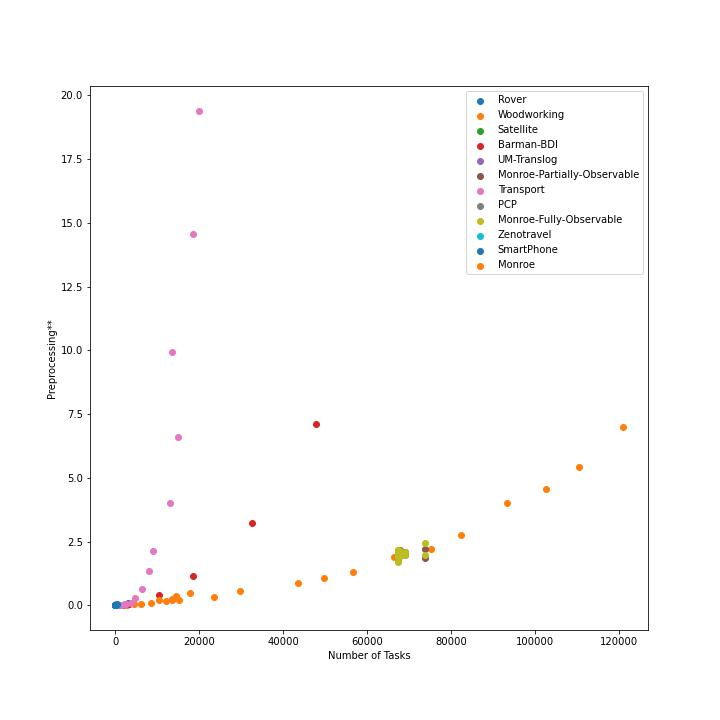
\includegraphics[scale=0.4]{../ipc2020-domains/Preprocessing**_vs_Tasksnotlog.jpg}
\end{center}

\begin{enumerate}
	\item None of the instances can be linearized.
	\item Despite this, ?percent of linearized problems are solvable.
	\item The additional processing time is within the same order of time as the time needed for grounding and a tiny fraction of the overall time $\sim$
	\item We compare the ratio of (Grounding + Pre-processing time + TO solve time) to (Grounding + PO solve time), as those
	are the steps needed to solve the respective problems. The average solve time for the TO problem is ?? percent of the PO problem, for all problems.
	\item Difference in reduction of total solving time influenced most by ? (e.g. domain, recursiveness of problem, percentage of linearizable methods, etc)
\end{enumerate}                              % evaluation
\chapter{Concluding Remarks}\label{chap:conclusion}

If you wish, you may also name that section \emph{``Conclusion and Future Work''}, though it might not be a perfect choice to have a section named ``A \& B'' if it has subsections ``A'' and ``B''. Also note that you don't necessarily have to use these subsections; that also depends on how much content you have in each. (E.g., having a section header might be odd if it contains just three lines.)


\section{Conclusion}

This chapter usually summarizes the entire paper including the conclusions drawn, i.e., did the developed techniques work? Maybe add why or why not. Also note that every single scientific paper has such a section, so you can check out many examples, preferably at top-tier venues, e.g., by your supervisor(s).


\section{Future Work}

On top of that, you could discuss future work (and make clear why that is future work, i.e., by which observations did they get justified?).

Note that future work in scientific papers is often not mentioned at all or just in a very few sentences within the conclusion. That should not stop you from putting some effort in. This will (also) show the examiner(s)/supervisor(s) how well you understood the topic or how engaged you are.
                              % conclusion

\appendix
\chapter{Appendix: Explanation on Appendices}\label{chap:appendix1}

You may use appendices to provide additional information that is in principle relevant to your work, though you don't want \emph{every reader} to look at the entire material, but only those interested.

There are many cases where an appendix may make sense. For example:
\begin{itemize}
  \item You developed various variants of some algorithm, but you only describe one of them in the main body, since the different variants are not that different.
  \item You may have conducted an extensive empirical analysis, yet you don't want to provide \emph{all} results. So you focus on the most relevant results in the main body of your work to get the message across. Yet you present the remaining and complete results here for the more interested reader.
  \item You developed a model of some sort. In your work, you explained an excerpt of the model. You also used mathematical syntax for this. Here, you can (if you wish) provide the actual model as you provided it in probably some textfile. Note that you don't have to do this, as artifacts can be submitted separately. Consult your supervisor in such a case.
  \item You could also provide a list of figures and/or list of tables in here (via the commands \verb!\listoffigures! and \verb!\listoftables!, respectively). Do this only if you think that this is beneficial for your work. If you want to include it, you can of course also provide it right after the table of contents. You might want to make this dependent on how many people you think are interested in this.
\end{itemize}
                              % appendix 1
\chapter{Appendix: Explanation on Page Borders}\label{chap:appendix2}

What you find here is an explanation of why the border width keeps flipping from left to right -- which you might have spotted and wondered why that's the case.

Firstly, that is \emph{intended} and thus correct, so there is no reason to worry about this. The reason is that this document is configured as a two-sided book, which means:
\begin{compactitem}
  \item We assume the document will be printed out,
  \item that this will be done in a two-sided mode (i.e., the document will be printed on both sides of each page), and
  \item that the bookbinding will be in the middle, just like in every book.
\end{compactitem}

When you open the book, there are three borders of equal size~$n$. This however requires that even pages have a border of $n$ on their left and $\frac{n}{2}$ on their right, and odd pages have a border of $\frac{n}{2}$ on their left and $n$ on their right. This is illustrated in Figure~\ref{fig:pageBorders}.

\begin{figure}[h]
  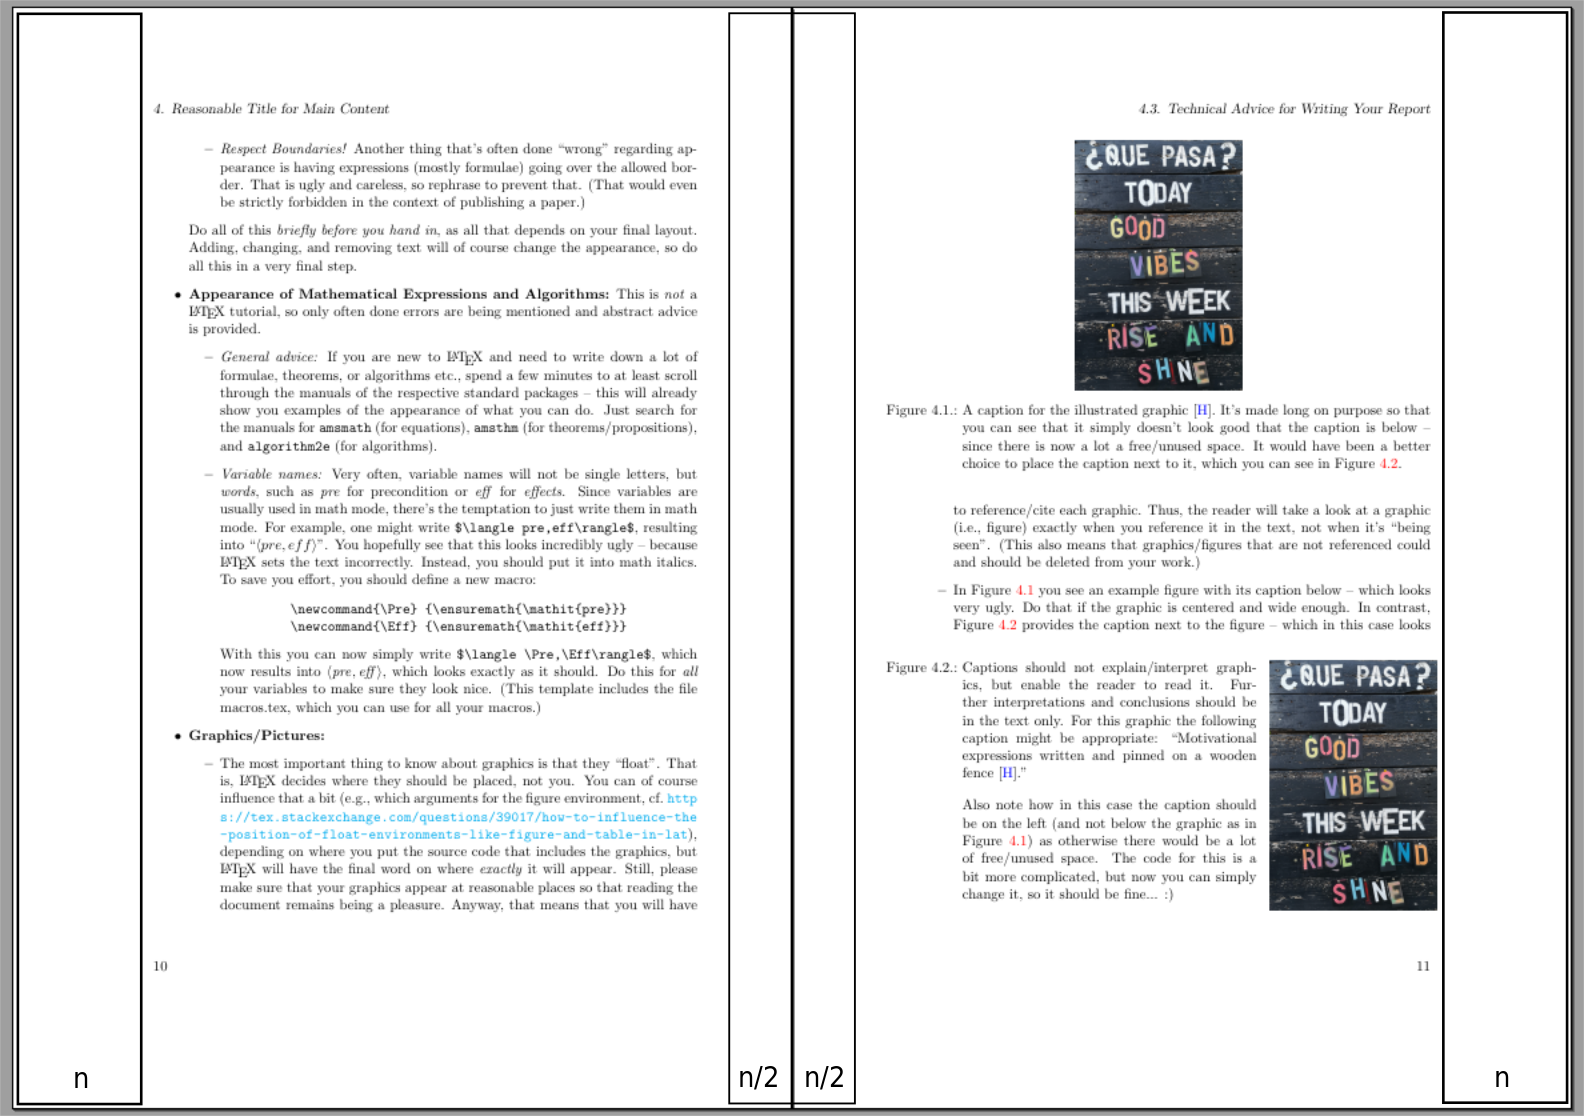
\includegraphics[width=.55\textwidth]{figures/borders--annotated}
  \caption{Illustration showing why page borders flip.\label{fig:pageBorders}}
\end{figure}%

                              % appendix 2


% literature
% \bibliographystyle{plainnat}
\bibliographystyle{anuthesis}
\bibliography{bib}
\end{document}
